
\documentclass[]{article}
\usepackage{ctex}
\usepackage{graphicx} 
%opening
\title{Behavior analysis using Resnet}

\author{Peizhi Wang}
\begin{document}

\maketitle

\begin{abstract}
This is simply a recording of my experiments on students behavior analysis.First week i will use Resnet to train all my training data.Then i will consider using transfer learning,data augmentation and other methods to build my model. 
\end{abstract}
\begin{CJK}{UTF8}{} 
\section{Introduction}
教育永远是一项非常重要的事业,是人类文明继承发展的主要方式。当今设备教育行业存在着如下几个问题:\\
1基础教育过分的注重考试成绩,给学生们增加了很大的压力\\
2大学教学只要考试合格就行,教育质量大大下滑\\
为了解决上述两个问题,一个非常可行的方向是记录学生的平时成绩和课堂活跃程度,这样既可以缓解基础教育同学们的考试压力,同时可以提高大学教育的质量。\\
但是,通过老师和助教来记录平时成绩是非常耗费精力的,而且由于部分助教不认识某些学生,就很难来记录学生的表现。如果点名的方式就会浪费珍贵的课堂时间。\\
然后,大学教室和大部分高中课堂是有着摄像头的。而今年的机器视觉又赋予了计算机来理解图片的能力。所以本文提出一种利用深度残差网络来对学生行为进行分类的方法,在复旦大学采集了一定量的数据集来进行训练和测试,取得了\\
还可以追踪学生的情绪,并且在学生情绪不佳的时候采取干预。\\
另外,通过对具有一定比例的学生的行为的分析,也可以用来评价老师的上课质量和学生对老师上课的满意程度。通过评教的方法是具有很大的误差,有时候学生也会因为被公开的评价会引起老师的生气,所以学生不容易在问卷调查中给出客观的评价。\\
\section{Patent using grading}
基于人脸和语音识别的课堂欣慰监控系统及方法
自动识别不同的教学场景
自动识别不同的上下课时间\\
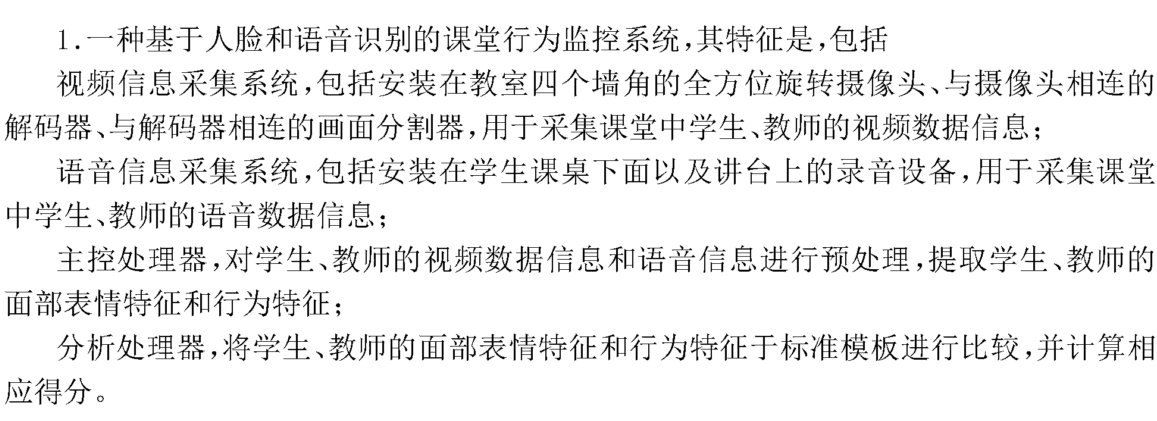
\includegraphics[width=5in]{pic1},\\
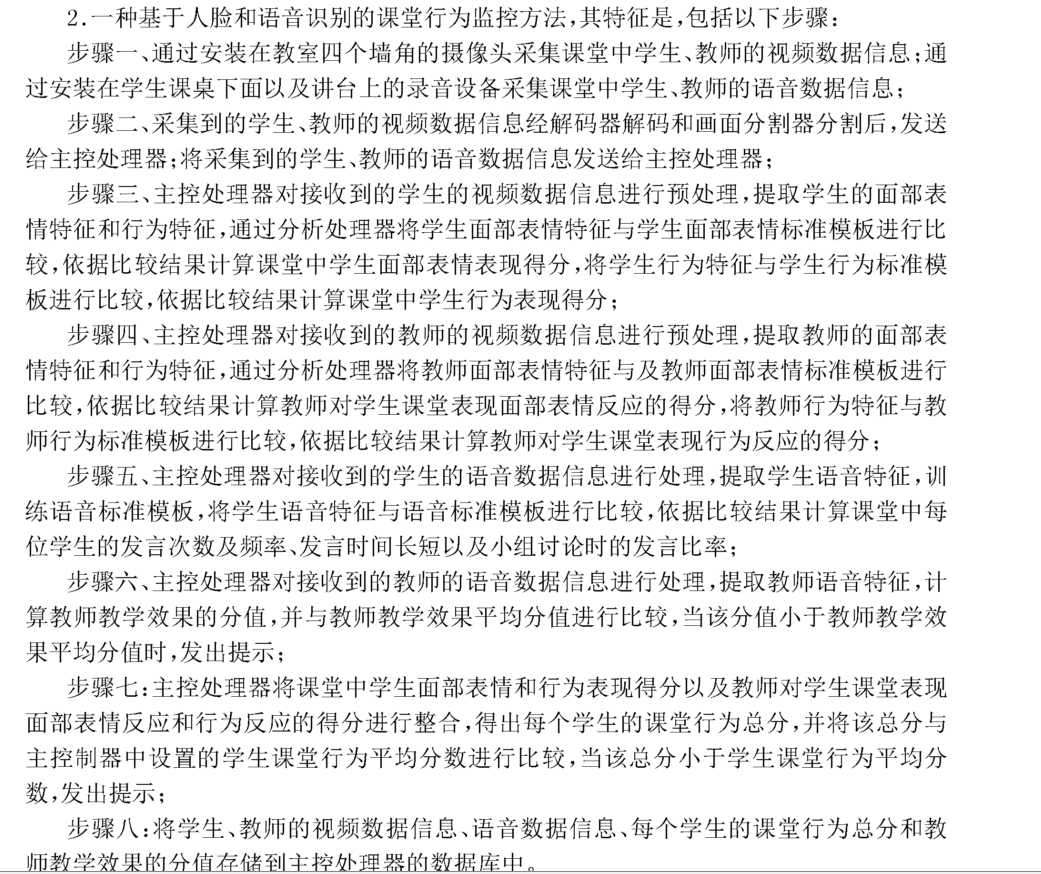
\includegraphics[width=5in]{pic2},\\

\includegraphics[width=5in]{pic3},\\
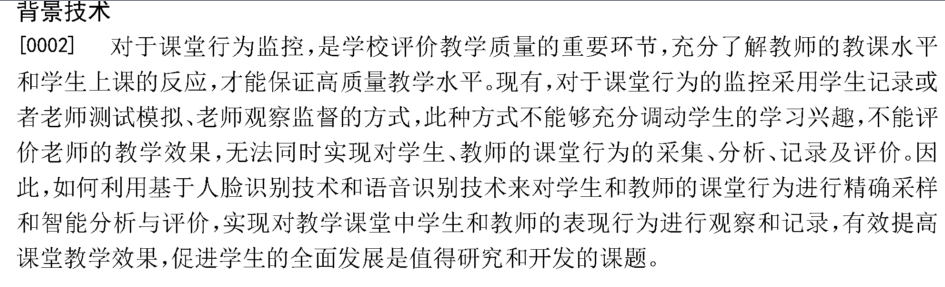
\includegraphics[width=5in]{pic4},\\
\section{Patent for teacher}
1将学生的评价数据采集起来,通过分析学生的行为,通过长期的累加,对教师的课堂教学质量进行评估。\\
在传统的教育活动中,人们往往过分强调老师教的作用,而忽略了学生听的效果,这种割裂教学的模式,往往造成学生积极性地下,缺乏上课的即使激励。然而现今教师的授课方式往往只有一名老师,在规定时间内对多名学生进行某一领域知识的教授。教师在有限的时间与精力下,并不能在课堂上完全了解每个学生对授课内容和质量的反应,为此,教师往往在课后对学生进行教学质量的调查。\\
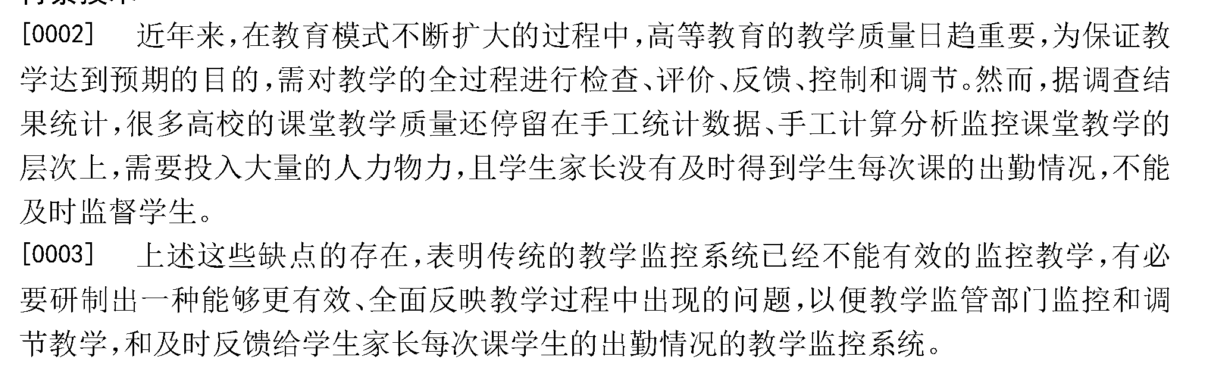
\includegraphics[width=5in]{pic9},\\
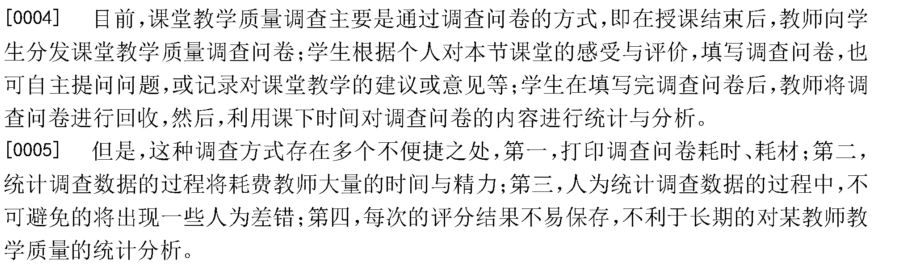
\includegraphics[width=5in]{pic5},\\
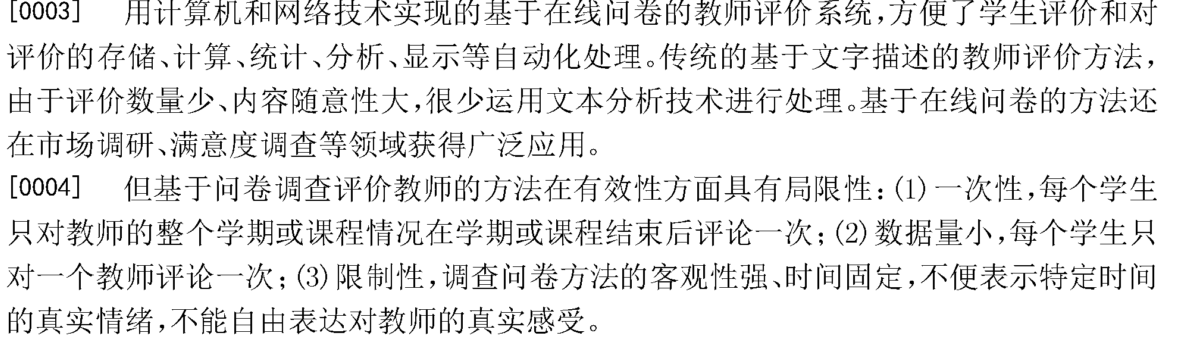
\includegraphics[width=5in]{pic6},\\
出于对机器视觉准确率的考量,所以就采用开心愉悦10分,冷漠4分,焦躁愤怒0分的打分制度。\\
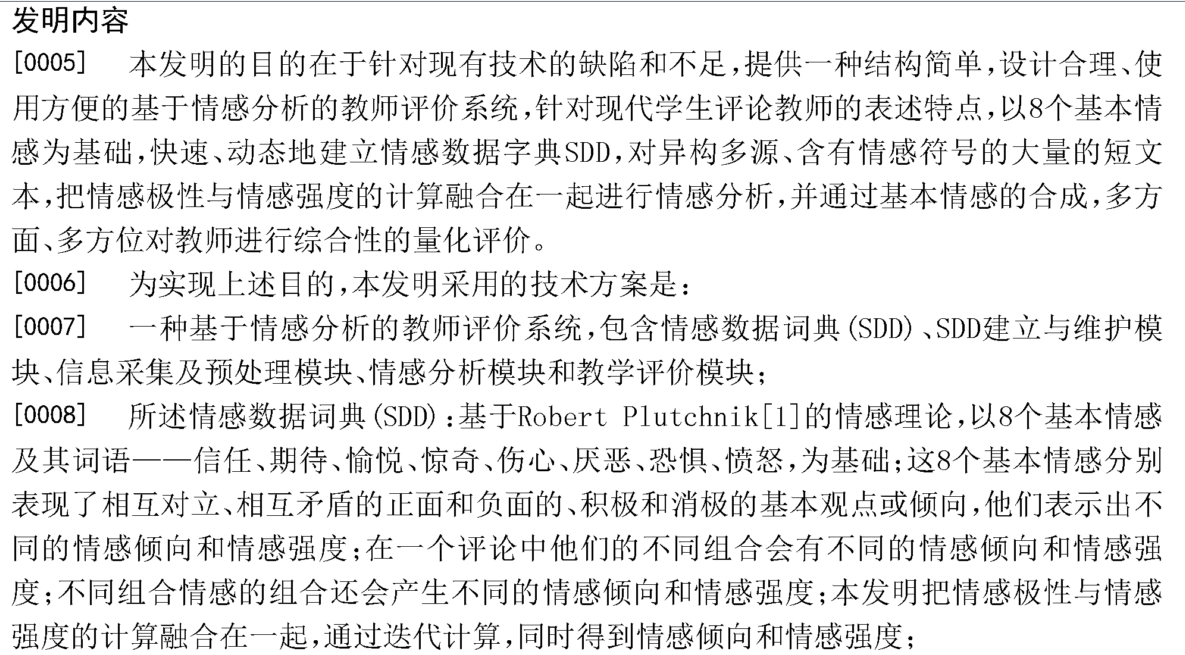
\includegraphics[width=5in]{pic7},\\
收集的信息包括文字,视频,音频,图像。这里考虑先进行图像的研究,然后拓展到视频方面。图片采样可以每0.1s采样一次,这样就可以有10FPS的照片数量。\\
获取班级位置的分布,比如是正三角,倒三角,均匀分布,前排空后排集中式等。通过分析学生上课历史的课堂特点,以及任课老师历史上课特点,定性来判断学生和老师的特点和行为。\\
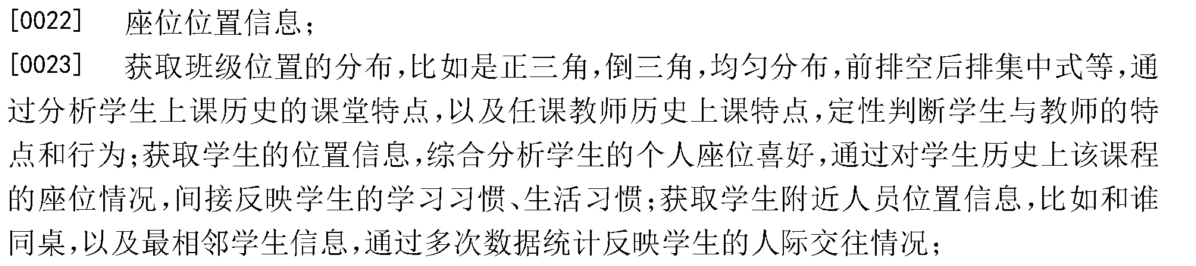
\includegraphics[width=5in]{pic8},\\
学生的表情,微笑或者严肃等,间接反映老师课堂中的兴奋点,课堂活跃程度。\\
检测学生是否处于睡眠状态,将信息反馈给教师,以便教师即使调整教学方法,教学内容以达到更好的教学效果,提高远程教学环境的交互性和教学质量。\\
智能教师现代远程教育的若干困难。\\
信息社会,只是爆炸,人们需要终身学习。这是个最好的时代,以网络为载体的远程教育顺应了这一趋势,给人们随时随地获取新知识提供了便利和强有力的支持。\\
但是这个方式也存在一些问题,比如学习是学生自发进行的,学生很难受到监督,这对于可以给出课程证书的远程课程就会减少其有效性。而且由于缺乏学生给与老师的即时反馈,老师也很难实时的发现学生在学习上存在的问题。\\
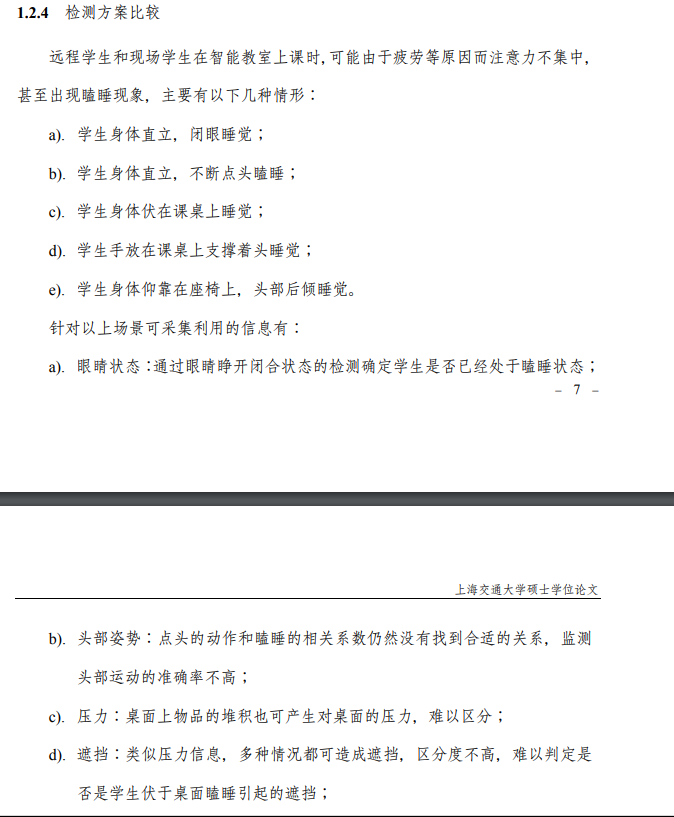
\includegraphics[width=5in]{pic10},\\
\section{Important multi hot code and split CNN}
想法的出发点是学生的动作肯定不是独立的.也就是说可以一边听课一边写作业,那么使用One-Hot编码的学生行为数目就比较小。\\
所以这里就放开One-hot的限制,使用Non maximun编码,也就是说让网络挑选出学生最有可能的至多三种行为,对于后面的行为我们就认为没有了。
一种proposal是采用多个神经网络对不同行为来进行分类。比如A网络来判决是否认真听课,B网络来判决是否有在吃东西,C网络判决是否睡觉。\\
后来我想了一种方法就是采用分叉CNN的方法,也就是一开始所有数据先经过一些网络层,提取出一部分特征,分布在M-Domain中,然后每个行为各自分叉一支出去。这样的好处有:\\
1网络的计算量变小了,共享了一部分的FP计算,视屏监控对实时性要求比较高\\
2网络具有更好的泛用性,借鉴了迁移学习的想法,形成一种共享学习的概念,可以减少对训练数据集合的要求。不然会随着任务数指数爆炸。\\
3网络具有更好的集成性,而不是单独的。\\
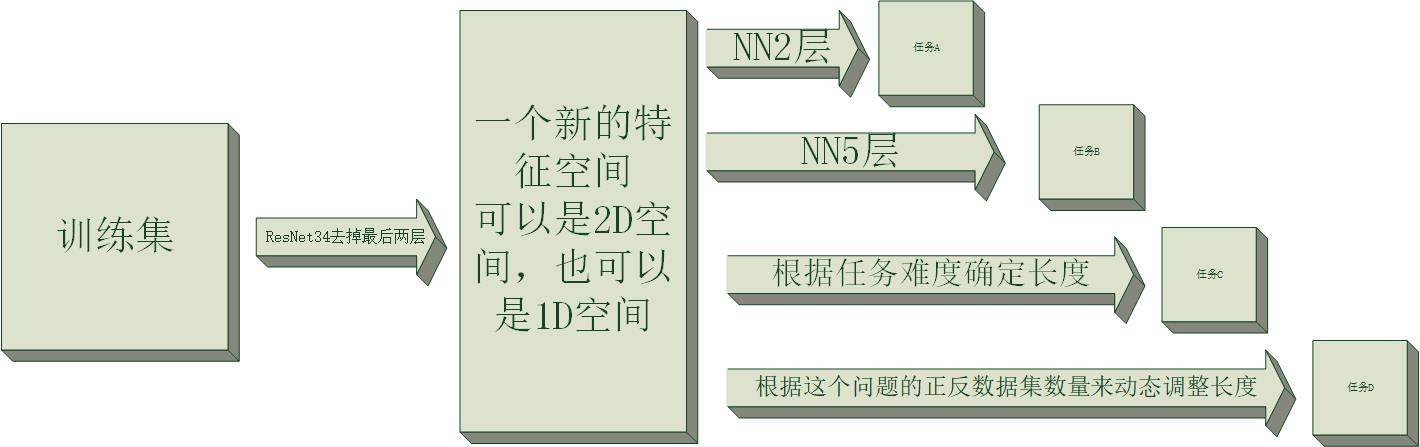
\includegraphics[width=5in]{TreeNN}, 
\section{Ideas}
可以加入学生的远景和近景,分辨学生的位置\\
可以加入学生的表情:happy,sad,没睡醒\\
可以加入学生的性别和身份识别\\
区分上下课:上课做的整整齐齐,下课都是随意走动\\
可解释性:统计大部分时间是0输出的神经元的个数,统计这个和Variance/Bias tradeoff的关系\\
我觉得可以尝试的一个方向是给教室里的每个学生做逐像素点的标记\\
\section{ZNN:Zoom Nerual Network}
我在想根据训练和测试图像,放大缩小结构大小或者卷积核大小\\
或者我在想能不能把卷积核弄成圆形的???\\
Inception 可以去看看\\
\section{Action Type}
根据某个观察量表,分为三大维度\\
一个是投入状态,包括一般倾听,举手发言等\\
另一个是非投入状态,包括看课外书,吃东西,玩手机,做作业,趴桌子,低头,使用PC电脑,喝水,左右交头接耳\\
另外还有课堂异常行为,包括缺席,中途站起离场或擅自走动,
\section{Action Recognition V1.0}
today i try to implement my first prototype V1.0.It is based on ResNet by(he kaiming).The training data is about 180 pictures about myself doing four kinds of actions.\\
without data augmentation,after 86 epochs,the training process was early stoped.
we get nearly 1.00 accuracy on training data and 0.90 accuracy on validation set,which is quite satisfying.\\
数据增强=False\\
使用了ResNet18
$$Rows=612$$
$$Cols=612$$
$$EarlySTOP = 87$$
$$acc_t=1$$
$$acc_v=0.9$$
主要是四个动作,睡觉写字玩手机听课
\section{Action Recognition V1.1}
数据增强=True 主要是每个图片的零均值单位方差,然后加上ZCA白化\\
使用了ResNet18
$$val/all=0.15$$
$$Rows=612$$
$$Cols=612$$
$$acc_t=$$
$$acc_v=$$
$$acc_t/sum=0.5$$
当我开启ZCA的时候,遇到了MEMORY ERROR,可能是在计算zca的时候会生成大矩阵的缘故吧\\
突然想到,也许可以比较一下远近的识别,也可以把近处的同学和远处的同学都区分开来,证明这个系统的泛用性。\\
第一次实验由于不小心early stop了,效果并不好。

\section{Action Recognition V1.2}
使用了ResNet34,观察网络层数增加的影响

\section{Action Recognition V2.0}
使用了新的数据集dataset2\\
A1 - A60 一边玩手机一边听音乐,低头\\
B1 - B58  一边看书一边听歌 ,低头\\
C1 - C55 站立,抬头\\
D1 - D62 举手,抬头\\
E1 - E60 抬头,喝水\\
F1 - F71 抬头,吃蛋糕\\
G1 - G60 抬头,写字\\
H1 - H55 一边看书一边写字\\
J1 - J67 一边玩手机一边看书\\
K1 - K52 吃东西,看书,低头\\
L1 - L70 低头,看书\\
M1 - M61 拿起手机在看\\
N1 - N66 趴着睡觉\\
O1 - O28 用手撑着睡觉\\
P1 - P37 抬头听课\\   

听音乐,水,食物,抬头,睡觉,写字,看书
\section{Action Recognition V3.0}
在这一个版本中,需要重新梳理一下我所需要的动作,然后开始写文章。\\
可以单独处理四种睡姿:\\
学生身体直立,闭眼睡觉;\\
学生身体伏在课桌上睡觉;\\
学生手放在课桌上支撑着头睡觉;\\
学生身体仰靠在座椅上,头部后倾睡觉。\\
单独处理三种表情:
开心激动 10分\\
冷漠 5分\\
焦躁不安 0分\\
单独处理是否吃东西喝水:\\
吃东西;2分\\
喝水; 5分\\
单独处理是否玩手机:\\
玩手机;\\
不玩手机。\\
单独处理是否看书写字:\\
看书 7分\\
写字 9分\\
单独处理是否听音乐:\\
戴着头戴式耳机 0分\\
没戴头戴式耳机 5分\\
单独处理是否举手:\\
举手 9分\\
不举手 5分\\
\section{Residual Network}
$$y_l=h(x_l)+F(X_l,W_l)$$
$$X_{l+1}=f(y_l)$$
\end{CJK}
\end{document}
